\documentclass[10pt]{beamer}
\usetheme{PaloAlto}
\usecolortheme{seahorse}
\setbeamertemplate{navigation symbols}{}
\setbeamertemplate{caption}[numbered]
%general package
%\usepackage[utf8]{inputenc}
\usepackage[english]{babel}
\usepackage{geometry}
\usepackage{tcolorbox}
\usepackage[export]{adjustbox}
\usepackage{graphicx}
\graphicspath{{../img/}}

%math package
\usepackage{amsmath}
\usepackage{amsfonts}
%\usepackage{amssymb}
%\usepackage{amsthm}
%\usepackage{slashed}
%\usepackage{tikz-cd}

%font package
%\usepackage{mathrsfs}
%\usepackage{bm}

%misc. package
\usepackage{enumitem}

\author[B.H.]{{\Large MATH211 Calculus III}\\\vspace{6pt}Instructor: Ben Huang}
\date{}
\title[Section 13.8]{Section 13.8 Extrema of Functions of Two Variables}
\institute[MU]{
\includegraphics[width = 0.382\textwidth]{MCLogo-Bck.png}}
\logo{
\includegraphics[scale = 0.3]{MCLogo-Bck.png}}
%general package
\usepackage[utf8]{inputenc}
\usepackage[english]{babel}
\usepackage{geometry}

%math package
\usepackage{amsmath}
\usepackage{amsfonts}
\usepackage{amssymb}
\usepackage{amsthm}
\usepackage{slashed}
\usepackage{tikz-cd}

%font package
\usepackage{mathrsfs}
\usepackage{bm}

%misc. package
\usepackage{enumitem}
\usepackage{tcolorbox}
\usepackage{etoolbox}
\usepackage{hyperref}
\hypersetup{
  colorlinks=true, urlcolor=blue
}




%declared operators
\DeclareMathOperator{\id}{Id}%identity
\DeclareMathOperator{\ind}{Ind\!}%index
\DeclareMathOperator{\tr}{Tr}%trace
\DeclareMathOperator{\e}{e}%exponential
\DeclareMathOperator{\im}{Im\!}%image
\DeclareMathOperator{\vol}{vol}%volume
\DeclareMathOperator{\cll}{\C\ell}%complexified Clifford algebra
\DeclareMathOperator{\gd}{\slashed{\partial}}%geometric Dirac
\DeclareMathOperator{\D}{\mathcal{D}}%generalized Dirac
\DeclareMathOperator{\Div}{div}%divergence
\DeclareMathOperator{\ud}{\,\mathrm{d}\!}

\DeclareMathOperator{\Hom}{Hom}
\DeclareMathOperator{\xd}{\,d\!}
\DeclareMathOperator{\curl}{curl}
\DeclareMathOperator{\dive}{div}


\newcommand{\norm}[1]{\lVert#1\rVert}
\newcommand{\R}{\mathbb R}
\newcommand{\vF}{\mathbf F}
\newcommand{\vv}{\mathbf v}
\newcommand{\inpr}[1]{\left\langle#1\right\rangle}
\newcommand{\fix}{(a,b)}
\newcommand{\uv}{\mathbf u}
\newcommand{\abs}[1]{\lvert #1\rvert}
%texting in citation
\makeatletter
\let\cite\relax
\DeclareRobustCommand{\cite}{%
  \let\new@cite@pre\@gobble
  \@ifnextchar[\new@cite{\@citex[]}}
\def\new@cite[#1]{\@ifnextchar[{\new@citea{#1}}{\@citex[#1]}}
\def\new@citea#1{\def\new@cite@pre{#1}\@citex}
\def\@cite#1#2{[{\new@cite@pre\space#1\if\relax\detokenize{#2}\relax\else, #2\fi}]}
\makeatother

\begin{document}
\frame{\titlepage}
\begin{frame}
\frametitle{Relative Extrema}
\begin{figure}
\centering
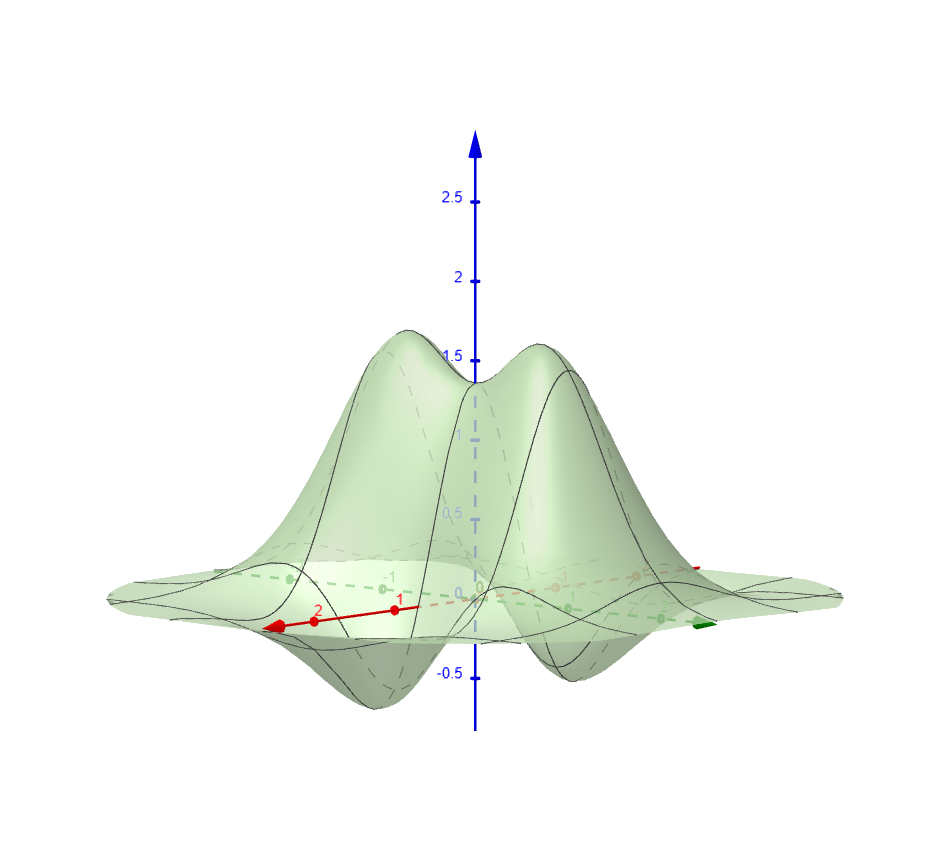
\includegraphics[width = 0.8\textwidth]{extrema2.png}
%\caption{$f(x.y) = (\frac{1}{2} - x^2 + y^2)\e^{1-x^2-y^2}$}
\end{figure}
\end{frame}


\begin{frame}
\frametitle{Relative Extrema}
\begin{figure}
\centering
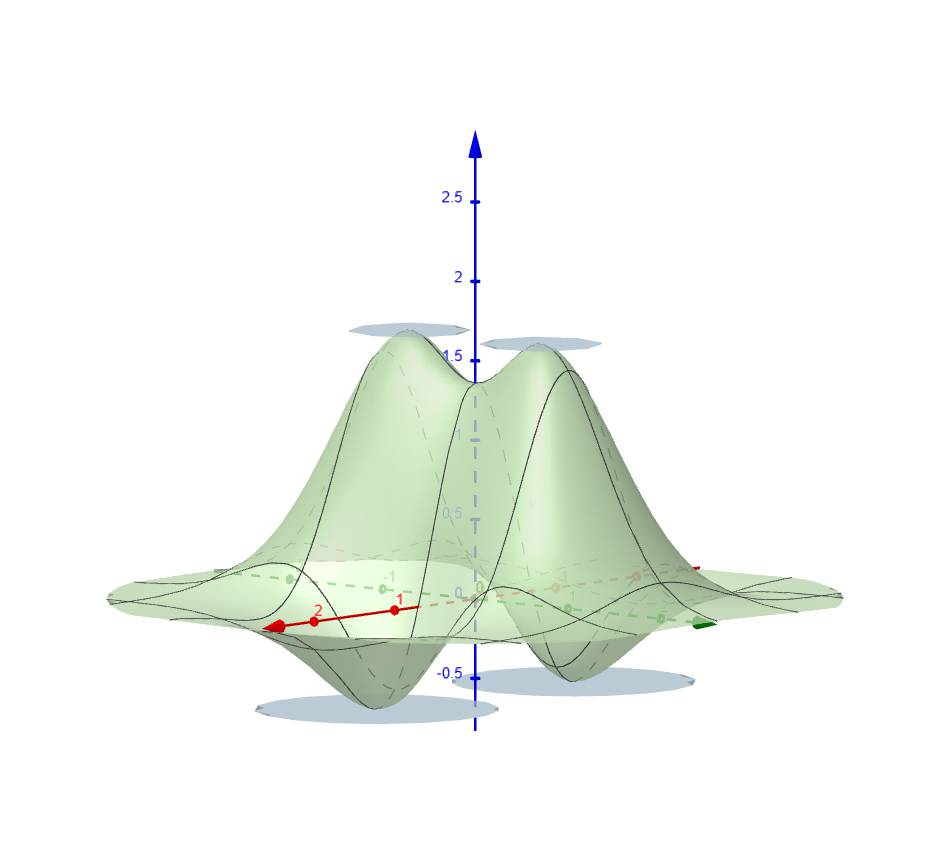
\includegraphics[width = 0.8\textwidth]{extrema1.png}
%\caption{$f(x.y) = (\frac{1}{2} - x^2 + y^2)\e^{1-x^2-y^2}$}
\end{figure}
\end{frame}

\begin{frame}
\frametitle{Critical points}
Where are the critical points?
\begin{tabular}{cc}
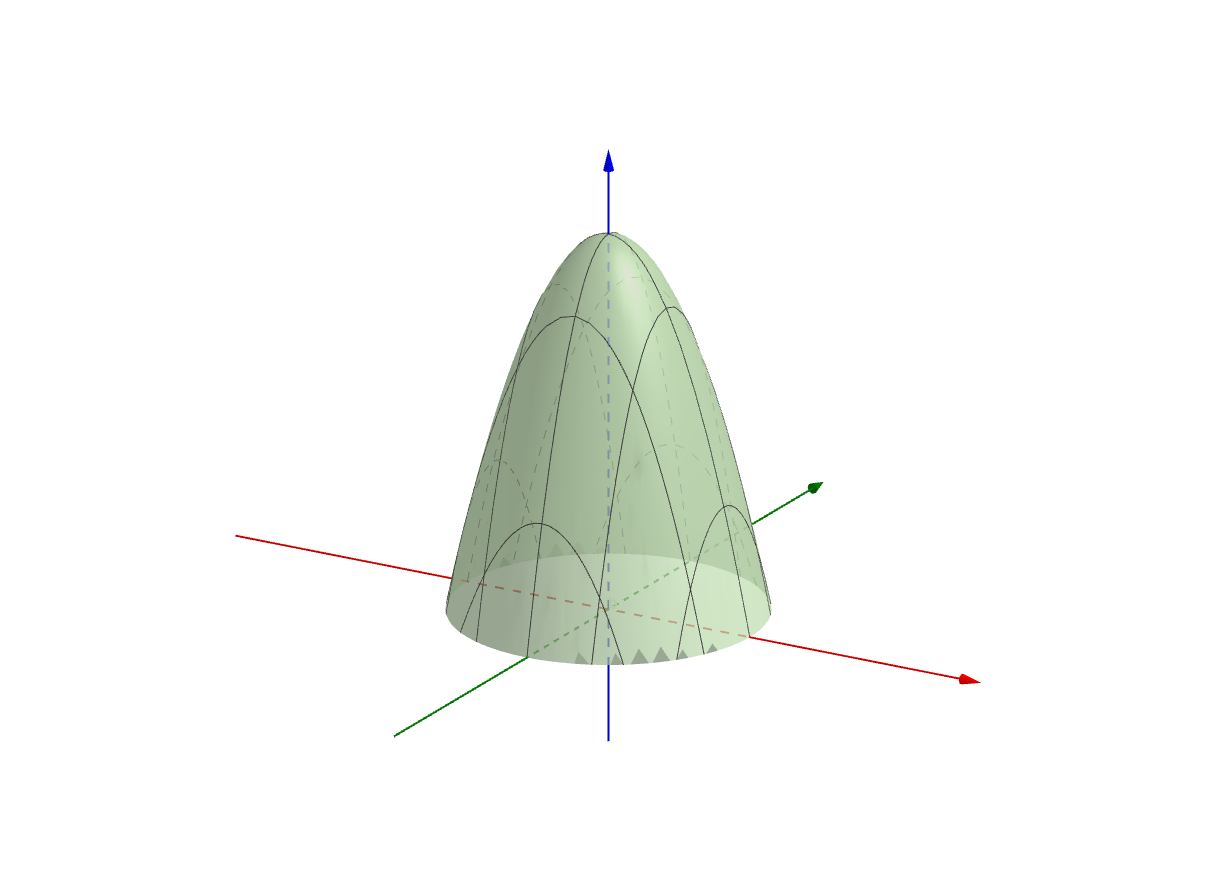
\includegraphics[width=0.45\textwidth]{max.png}&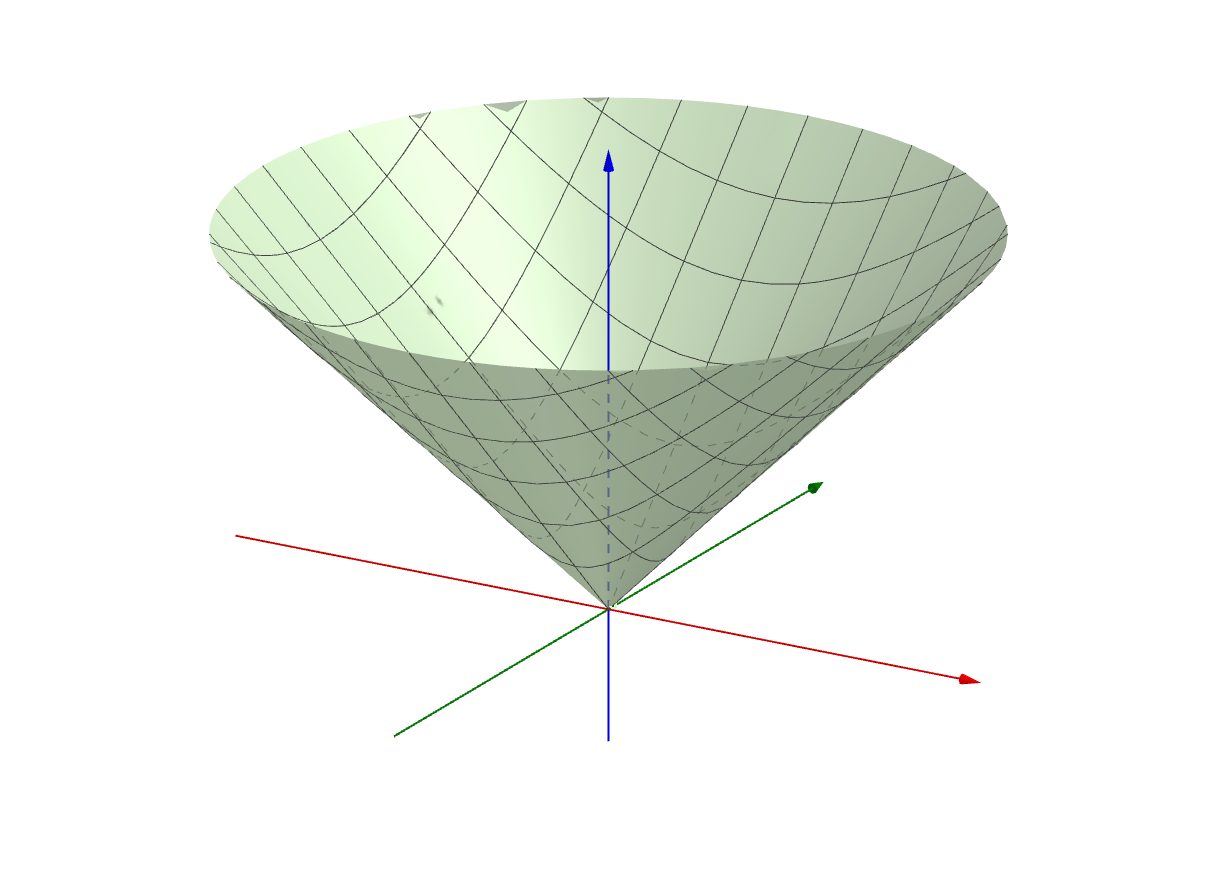
\includegraphics[width=0.45\textwidth]{cone.png}\\
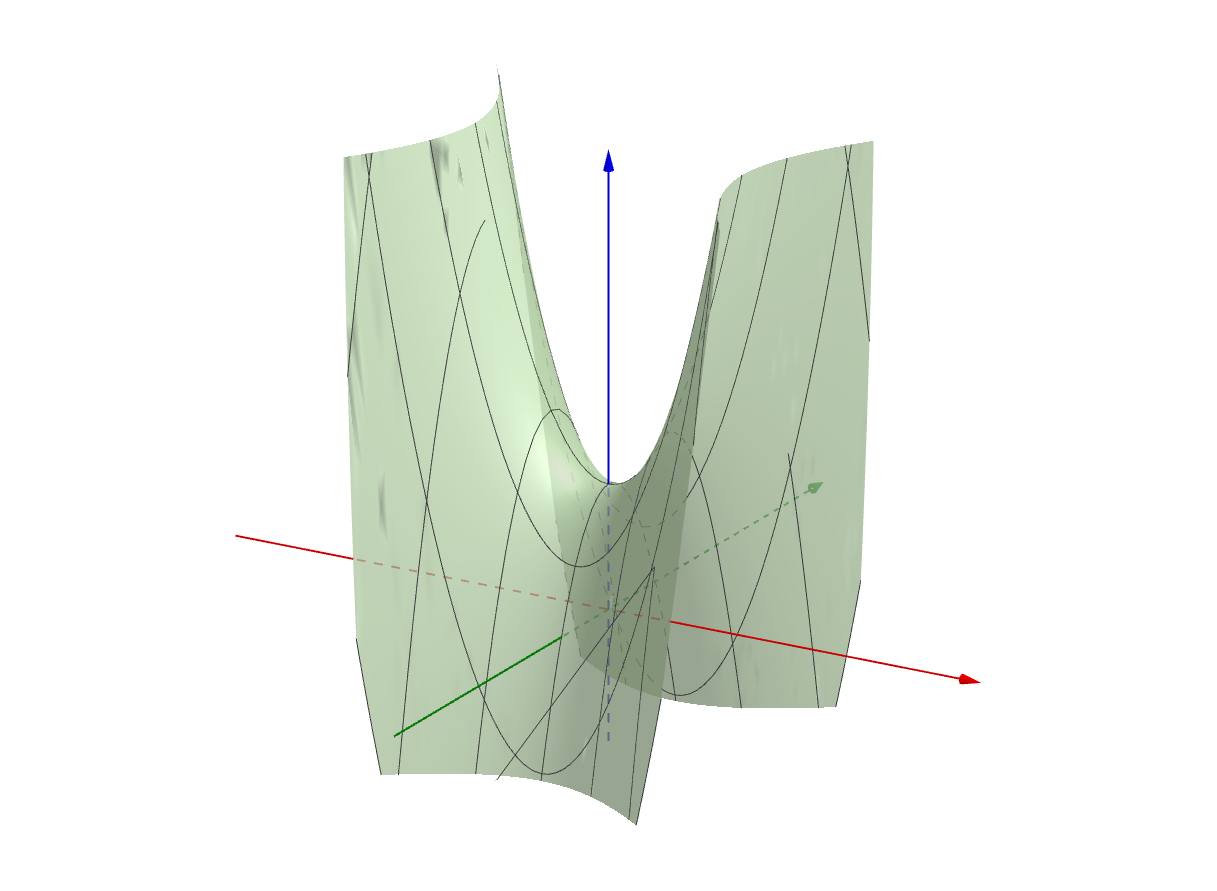
\includegraphics[width=0.45\textwidth]{saddle.png}&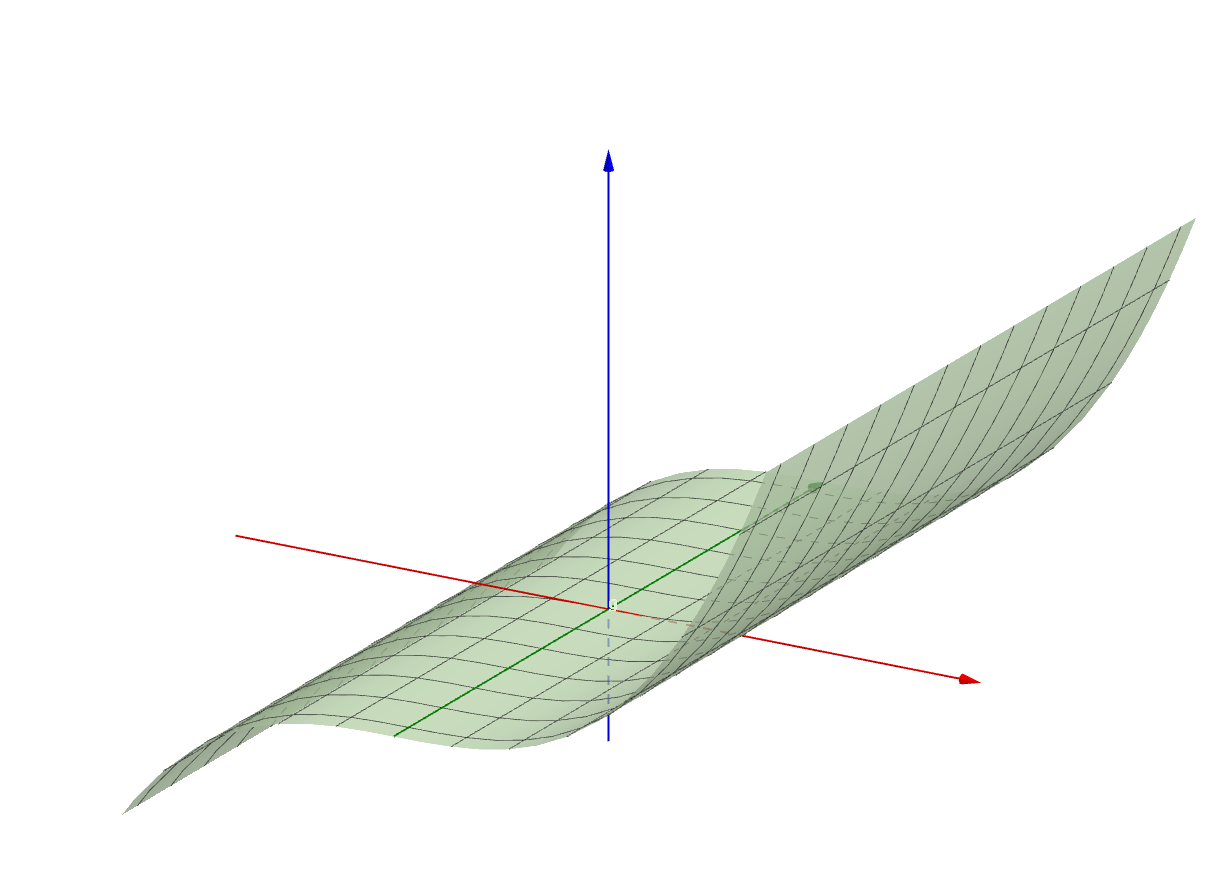
\includegraphics[width=0.45\textwidth]{fail3.png}
\end{tabular}
\end{frame}

\begin{frame}
\frametitle{Critical points}
Where are the critical points?
\begin{tabular}{cc}
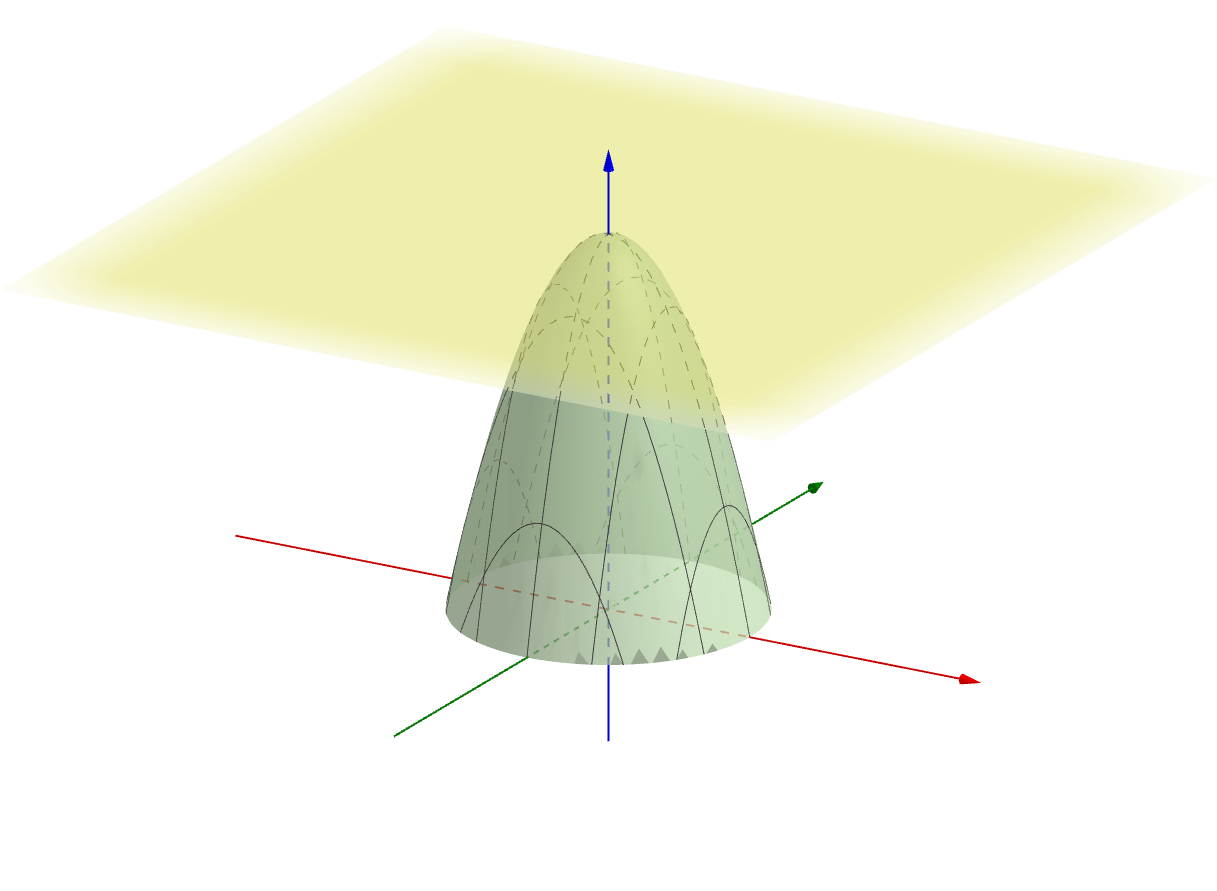
\includegraphics[width=0.45\textwidth]{max2.png}&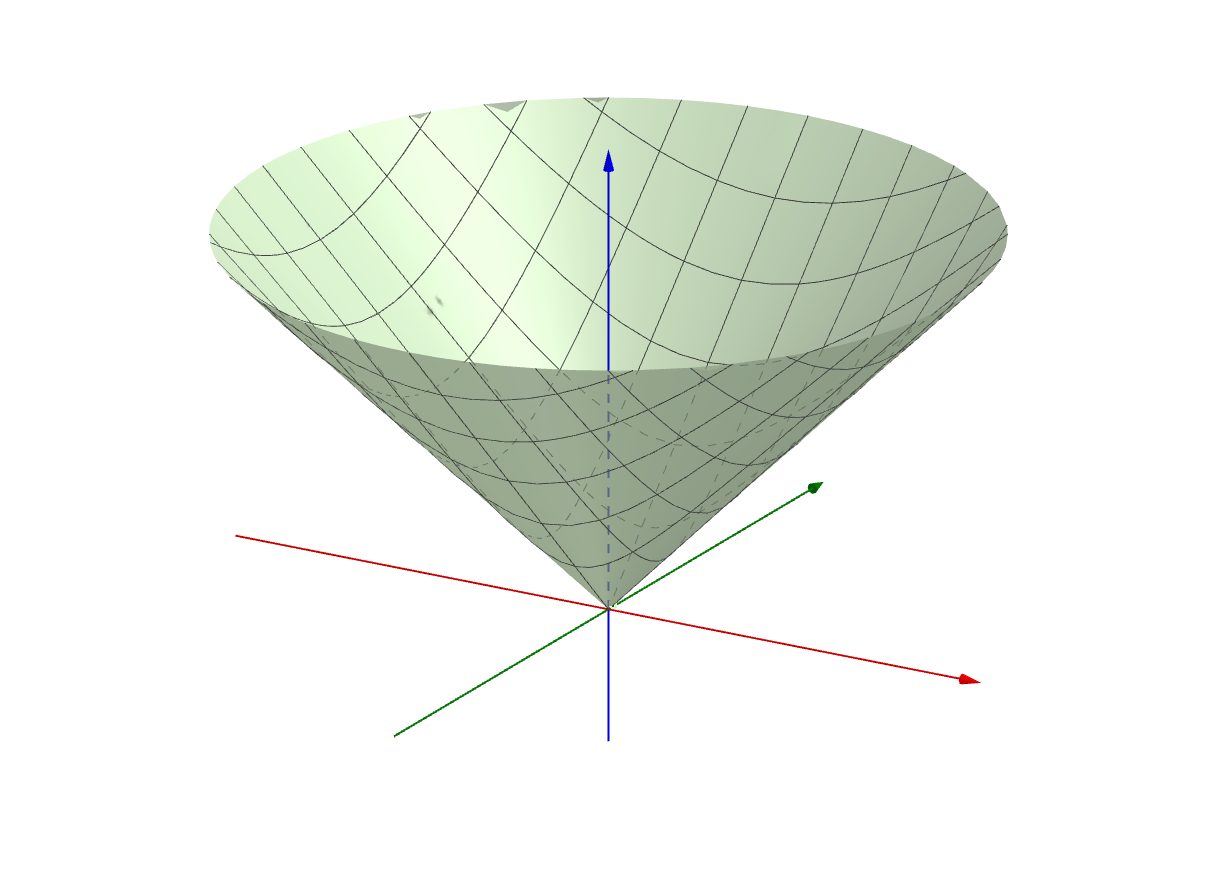
\includegraphics[width=0.45\textwidth]{cone.png}\\
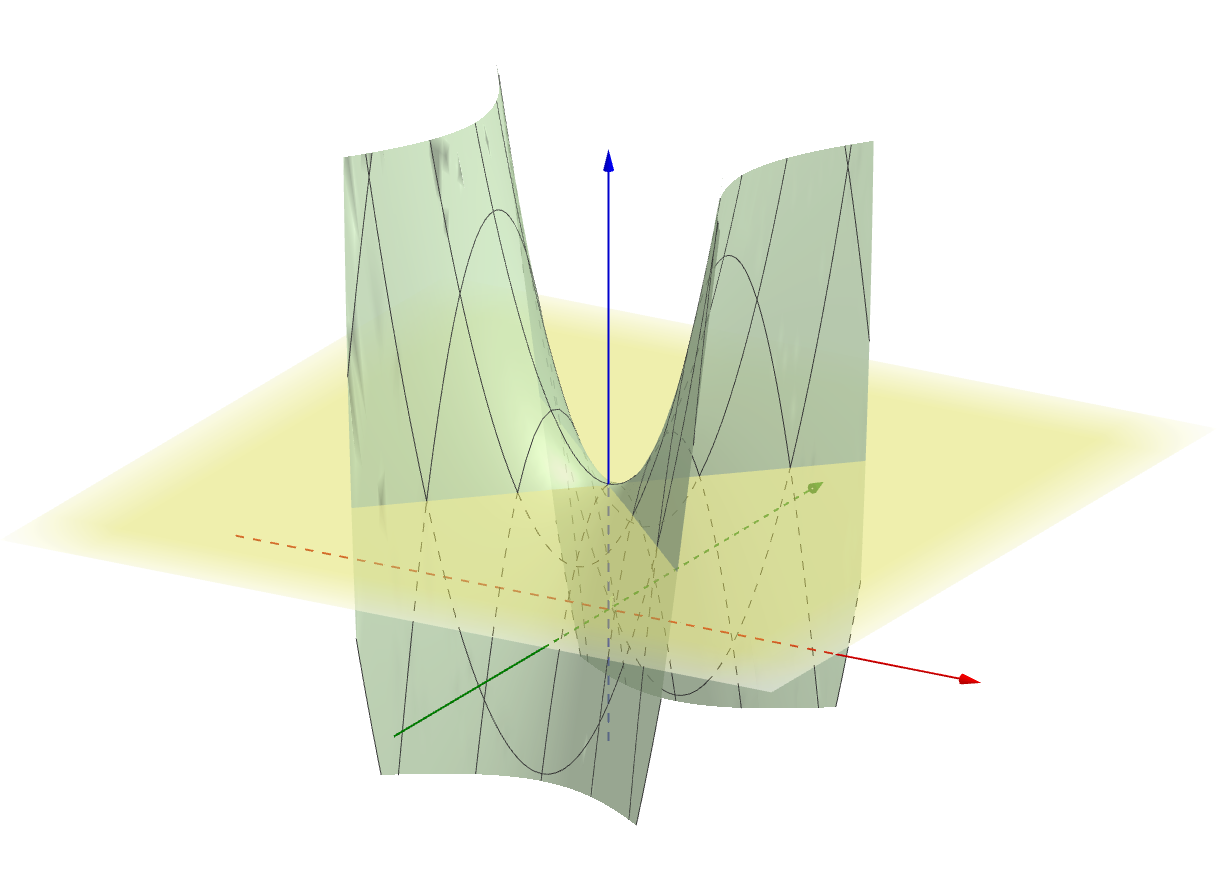
\includegraphics[width=0.45\textwidth]{saddle2.png}&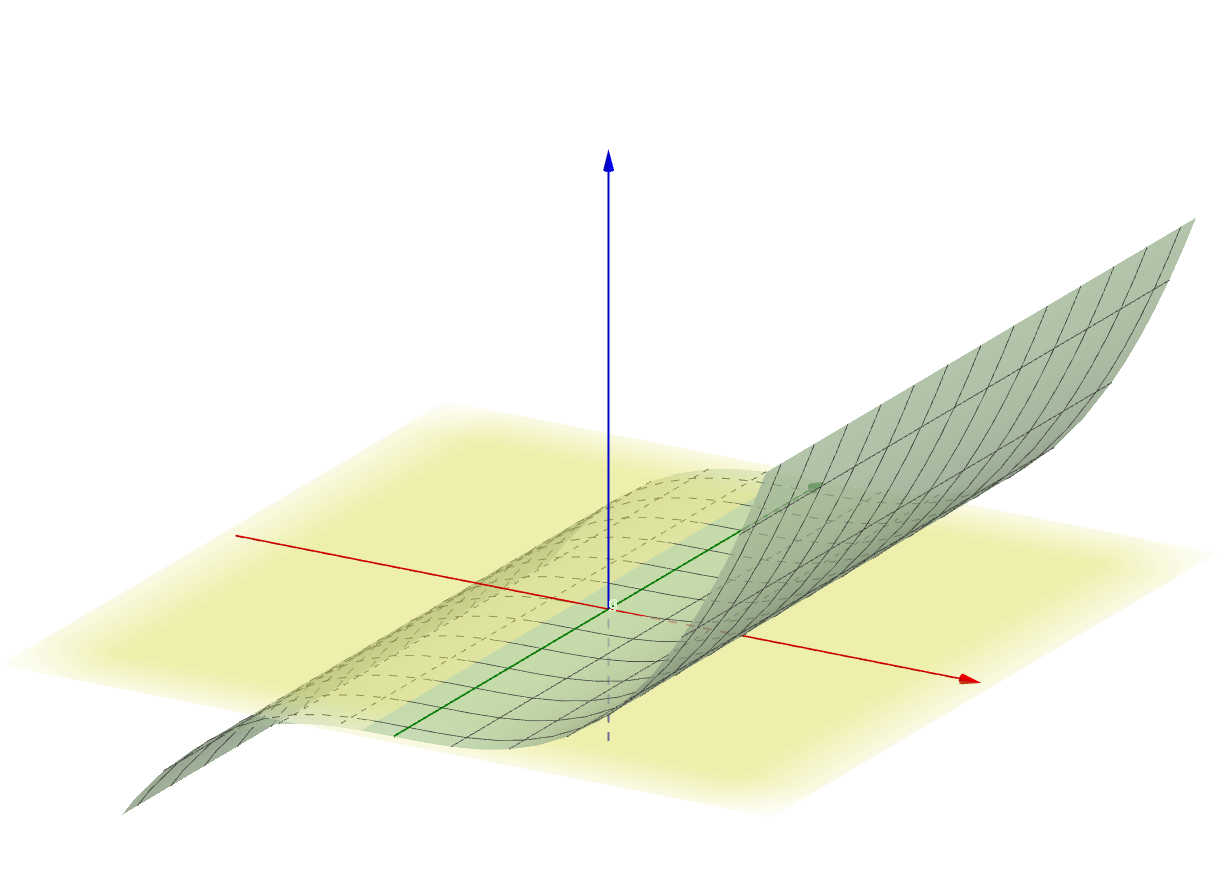
\includegraphics[width=0.45\textwidth]{fail32.png}
\end{tabular}
\end{frame}

\begin{frame}
\frametitle{Second Derivative Test From Calculus I}
\centering
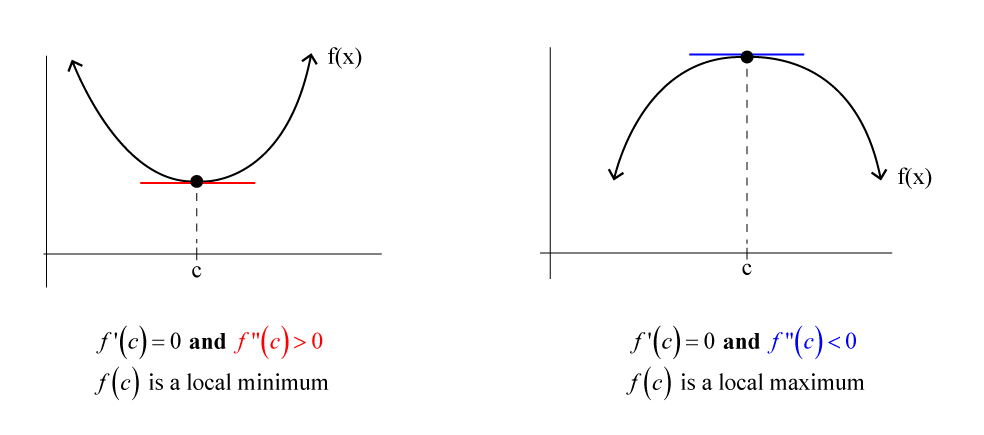
\includegraphics[width=\textwidth]{secondderivativetest.png}
\end{frame}

\begin{frame}
\frametitle{Classification of Critical Points}
\centering
\begin{tabular}{cc}
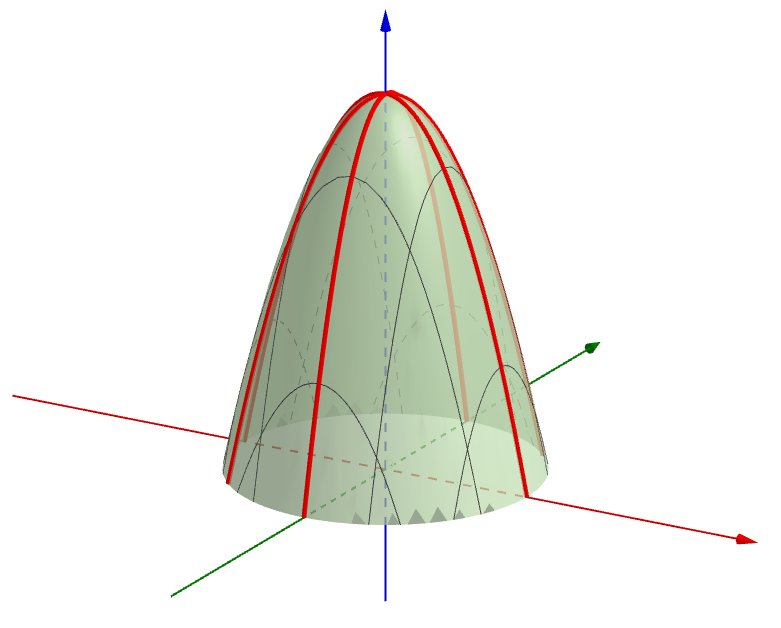
\includegraphics[width=.45\textwidth]{max3.png}&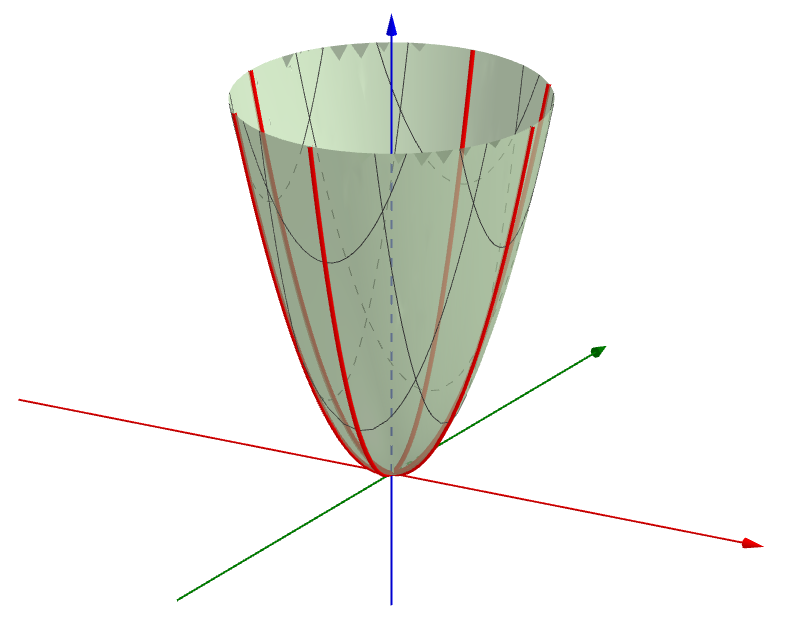
\includegraphics[width=.45\textwidth]{min3.png}\\[6pt]
\parbox{.45\textwidth}{\centering $f_{xx} < 0\ \&\ f_{yy} < 0$\\at the critical point\\local maximum} &\parbox{.45\textwidth}{\centering $f_{xx}>0\ \&\ f_{yy}>0$\\at the critical point\\local minimum}
\end{tabular}

\end{frame}

\begin{frame}
\frametitle{Classification of Critical Points}
\centering
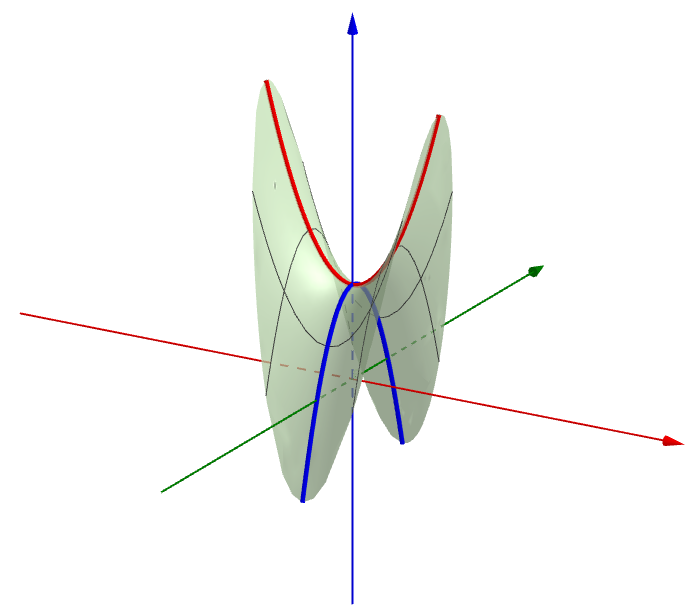
\includegraphics[width=.7\textwidth]{saddle3.png}

$f_{xx} >0\ \&\ f_{yy} < 0$ at the critical point

saddle point

\end{frame}

\begin{frame}
\frametitle{Classification of Critical Points}
\centering
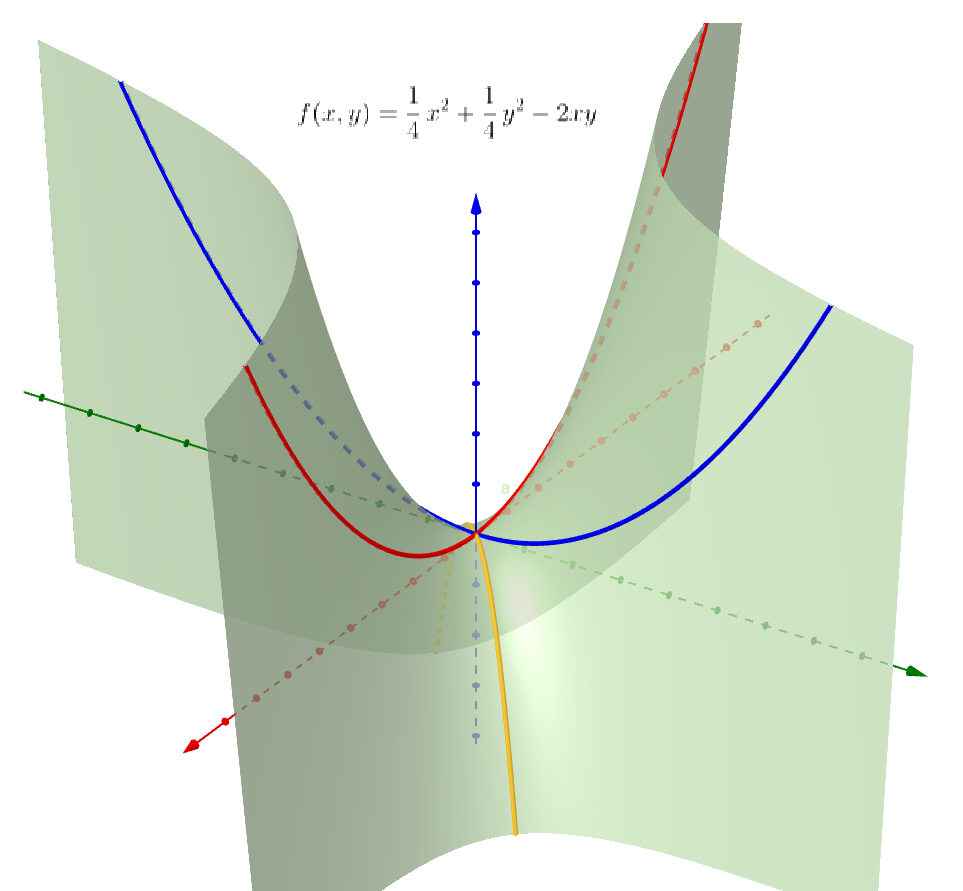
\includegraphics[width=.65\textwidth]{saddlepoint.png}
\vspace{\stretch{1}}

$f_{xx} >0\ \&\ f_{yy} > 0$ at the critical point

saddle point
\end{frame}

\begin{frame}
\frametitle{The Second Partials Test}
The tool to systematically classify critical points:
\href{https://ng.cengage.com/static/nb/ui/evo/index.html?eISBN=9780357749340&id=1514756126&snapshotId=2988231&}{The Second Partials Test}
\end{frame}

\begin{frame}
\frametitle{Failure of the Second Partials Test}
When $d(x,y) = f_{xx}f_{yy} - f_{xy}^2 = 0$ at the critical point in question, the Second Partials Test is {\bf inconclusive}.

\hspace{-1em}
\begin{minipage}{\textwidth}
\begin{columns}
\column{0.25\paperwidth}
\begin{figure}
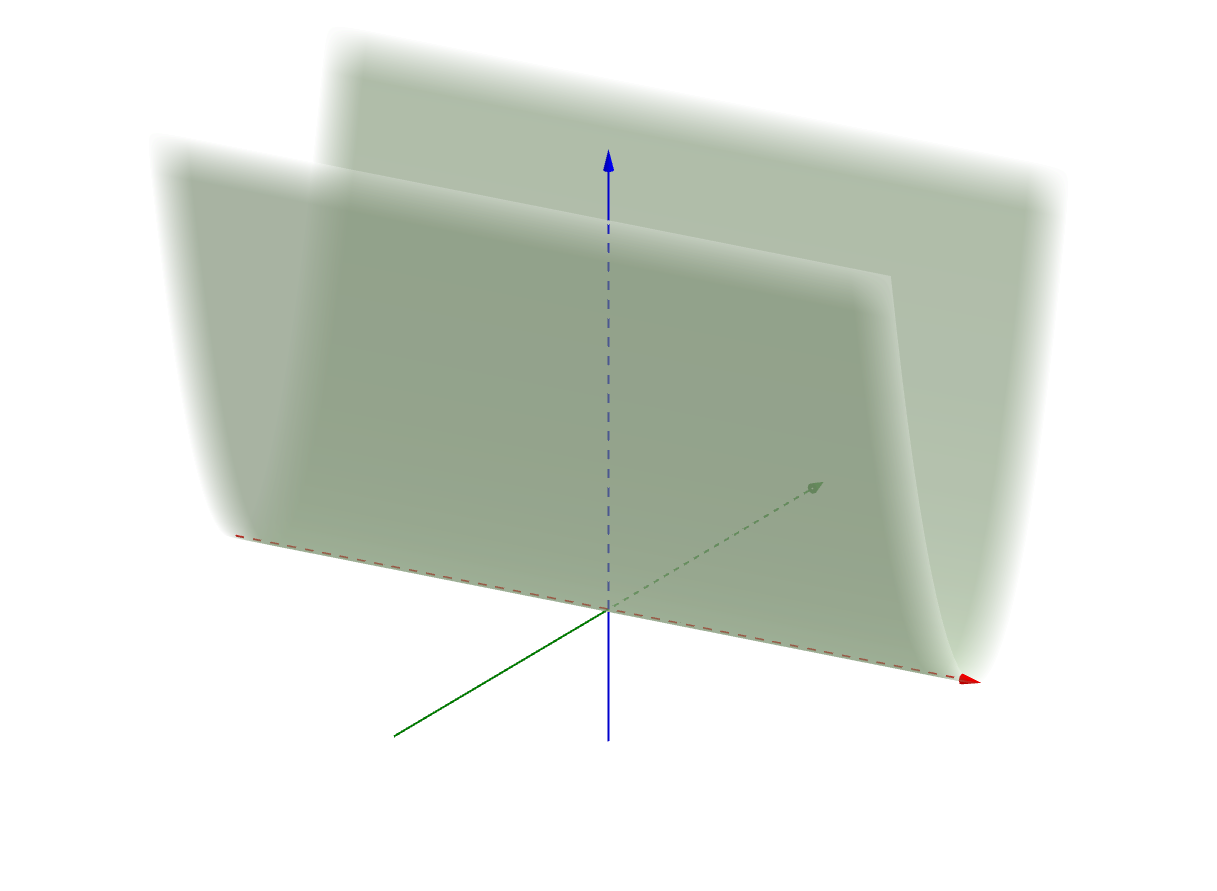
\includegraphics[width = 0.25\paperwidth]{fail.png}
\caption{$z=y^2$}
\end{figure}
\column{0.25\paperwidth}
\begin{figure}
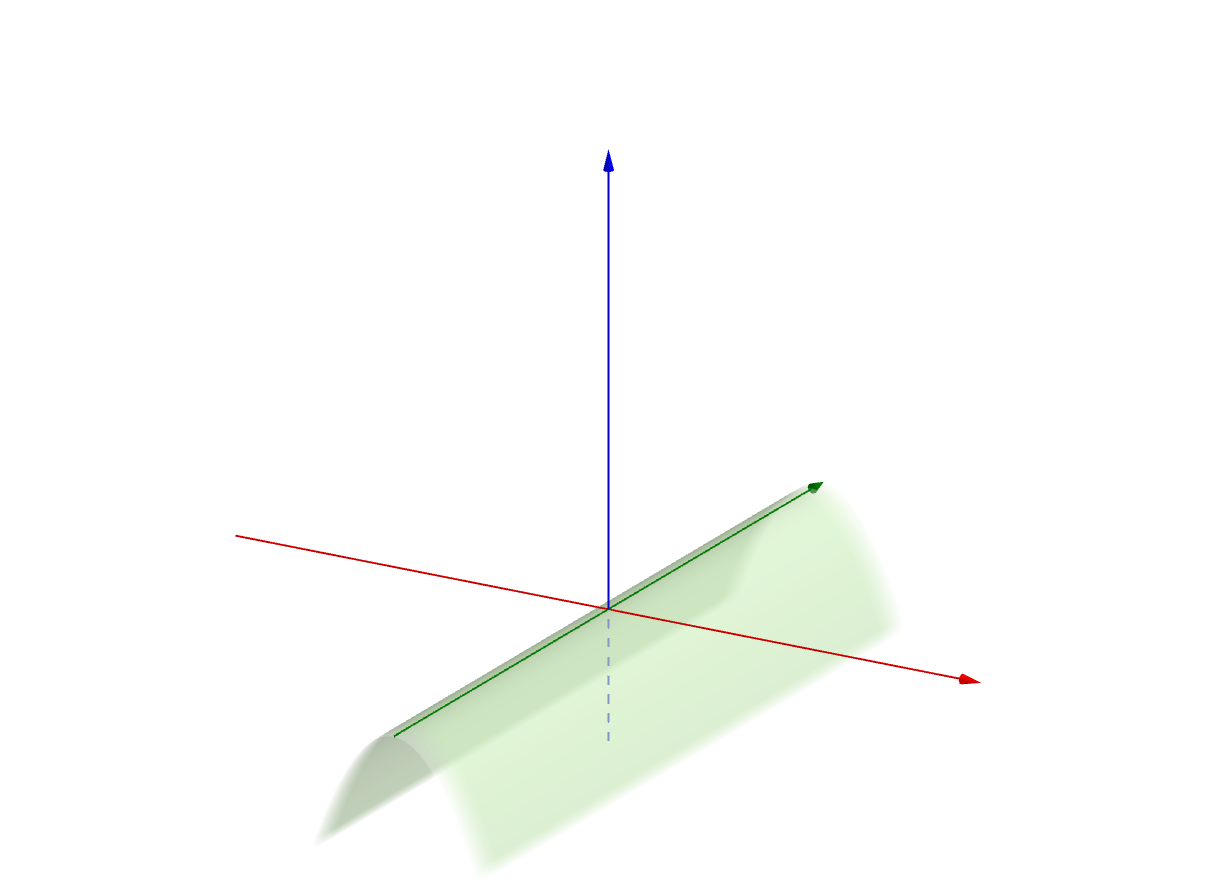
\includegraphics[width = 0.25\paperwidth]{fail2.png}
\caption{$z = -x^2$}
\end{figure}
\column{0.25\paperwidth}
\begin{figure}
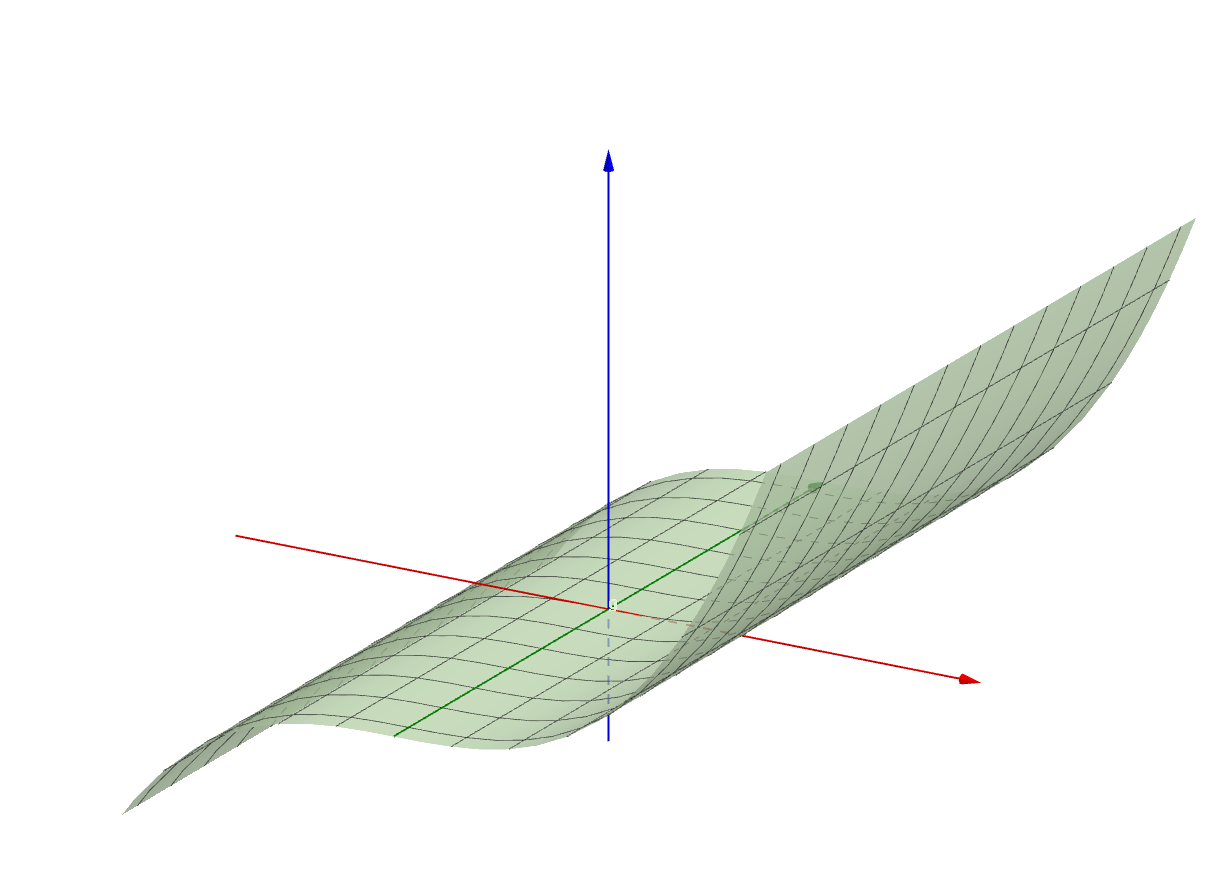
\includegraphics[width = 0.25\paperwidth]{fail3.png}
\caption{$z = \frac{1}{50}	x^3$}
\end{figure}
\end{columns}
\end{minipage}
\end{frame}
\end{document}